\chapter{Blockchain as the infrastructure of semantic web}

\section{Distributed ledgers and indexing}
A distributed ledger based on a blockchain does not have central control. Blockchains are organized into multiple blocks that initial block created manually and the other blocks are added by some consensus process between nodes.
Ethereum smart contract provides the possibility to control automatically what happens with cryptocurrency on the blockchain without involving the untrusted external sources. Ethereum smart contracts have an account that can normally store, update, or make a function with the input and output.
The concept\textit{accounts} are widely used in this study refer to an agent such as human and the concept \textit{balance} refers to cryptocurrency in blockchains. \\ 
As already said, smart contracts are time-ordered where data are stored into blocks. therefore it requires the data to index. Indexing the smart contract gives us the capability to access the data, search, analyze services on the distributed ledger and expose them to outside the worlds for more of interactions.
There are different levels of indexing smart contracts: Basic level is the fundamental level for the next step. It indexes basic entities such as account, blocks related to distributed level, and data can be stored or retrieved here. In the functional level, smart contracts contain a lot of functional interfaces that depict the other functionality of platforms such as Ethereum \cite{Third}. 

\subsection{Why do we use ontology for Blockchain?}

Generally, Blockchain is the distributed database that replicated over all nodes as a cloud computing architecture. These databases are distributed across multiple organizations. That's why standard interpretation is needed that the data would be understandable for organizations. Interpretations are applicable via formal specification that enables verification and inference within software and applications executed on the network. \\
This is where ontology comes to play to ensure a common interpretation of data of shared database among different enterprises.
blockchain as a modeling form used a different type of ontology: \\
\textbf{\textit{informal/semi ontology}} to facilitate search and enhance better understanding of the business process for developing and applying on the blockchain.\\
\textbf{\textit{Formal ontology}} helps the formal specification to automate inference and verify the operation of the blockchain. On the other word, blockchain modeling based on formal ontology can help the development of smart contract to execute on the blockchain.\\
Also, we can use ontology to capture data within blockchain: On one hand, It facilitates a better understanding of blockchain concepts for human. On the other hand, enables interlinking with other link data to convey deductions and formal reasoning\cite{Matthew}.\\
Vocabulary used within ontology increase the transparency of transaction in a way that by describing the transaction in the context of linked data comfort the graphical representation of the location of such transaction. Thus, it increases also the capability of analysis by users.

\begin{center}
	
	
	\begin{figure}[htb!]
		
		\begin{minipage}{0.55\linewidth}
			\centering
			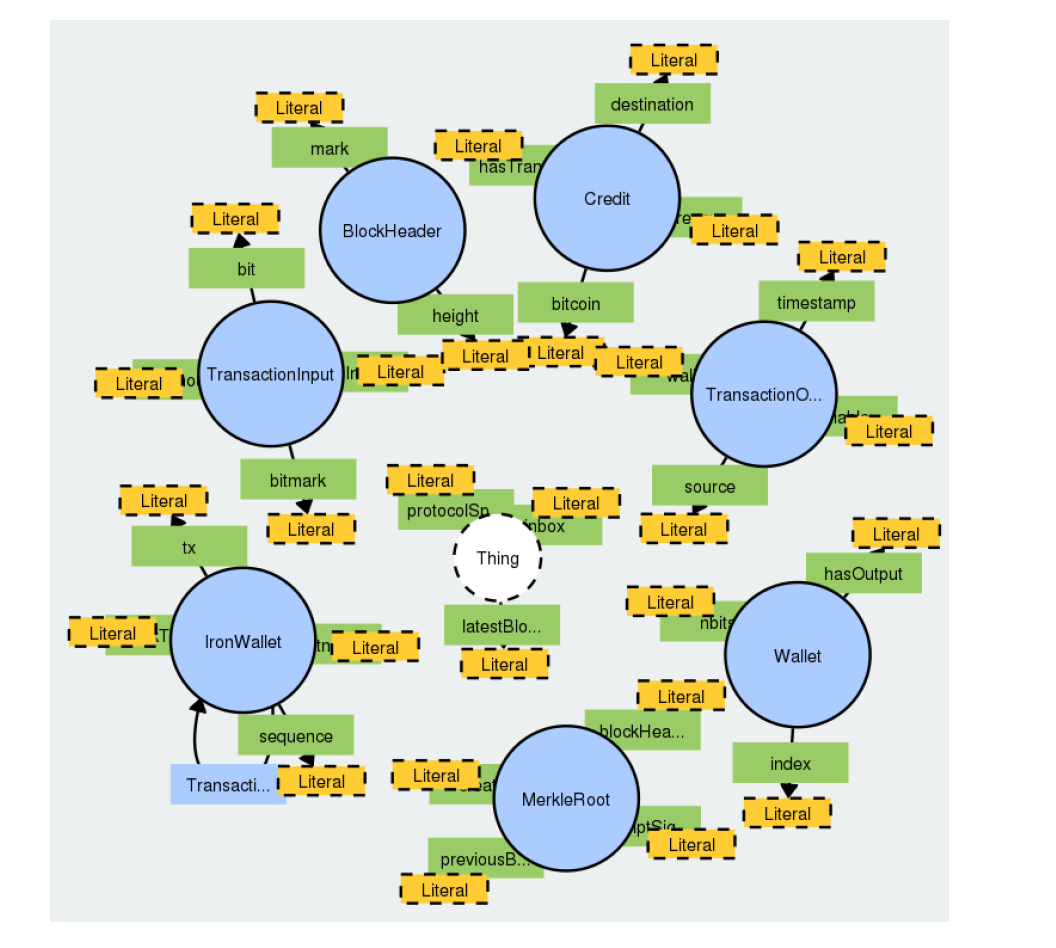
\includegraphics[width=1.65\textwidth]{images/chap02_diagram_ontology.png}
		\end{minipage}
		\caption[Illustration of Ontology diagram]{Illustration of Ontology diagram\cite{Matthew}}
		
		
	\end{figure}
	
\end{center}

\subsection{Linked Data}
Linked data is structure using vocabularies like schema.org to interlinked between different data and resources and it helps the semantic query of data. When information represents in linked data, querying about related information can be easily discovered. It is built up to standard web technologies such as \\
\textbf{- URIs}(Uniform Resource identifier) as names.\\ 
\textbf{- HTTP} to search for names.\\
\textbf{- (SPARQL, RDF)}  when a user search for something, provides related information.\\
\textbf{- Link} to other URLs to provide more information\cite{Hector}.\\

\begin{center}
	\begin{figure}[htb!]
		
		\begin{minipage}{0.55\linewidth}
			\centering
			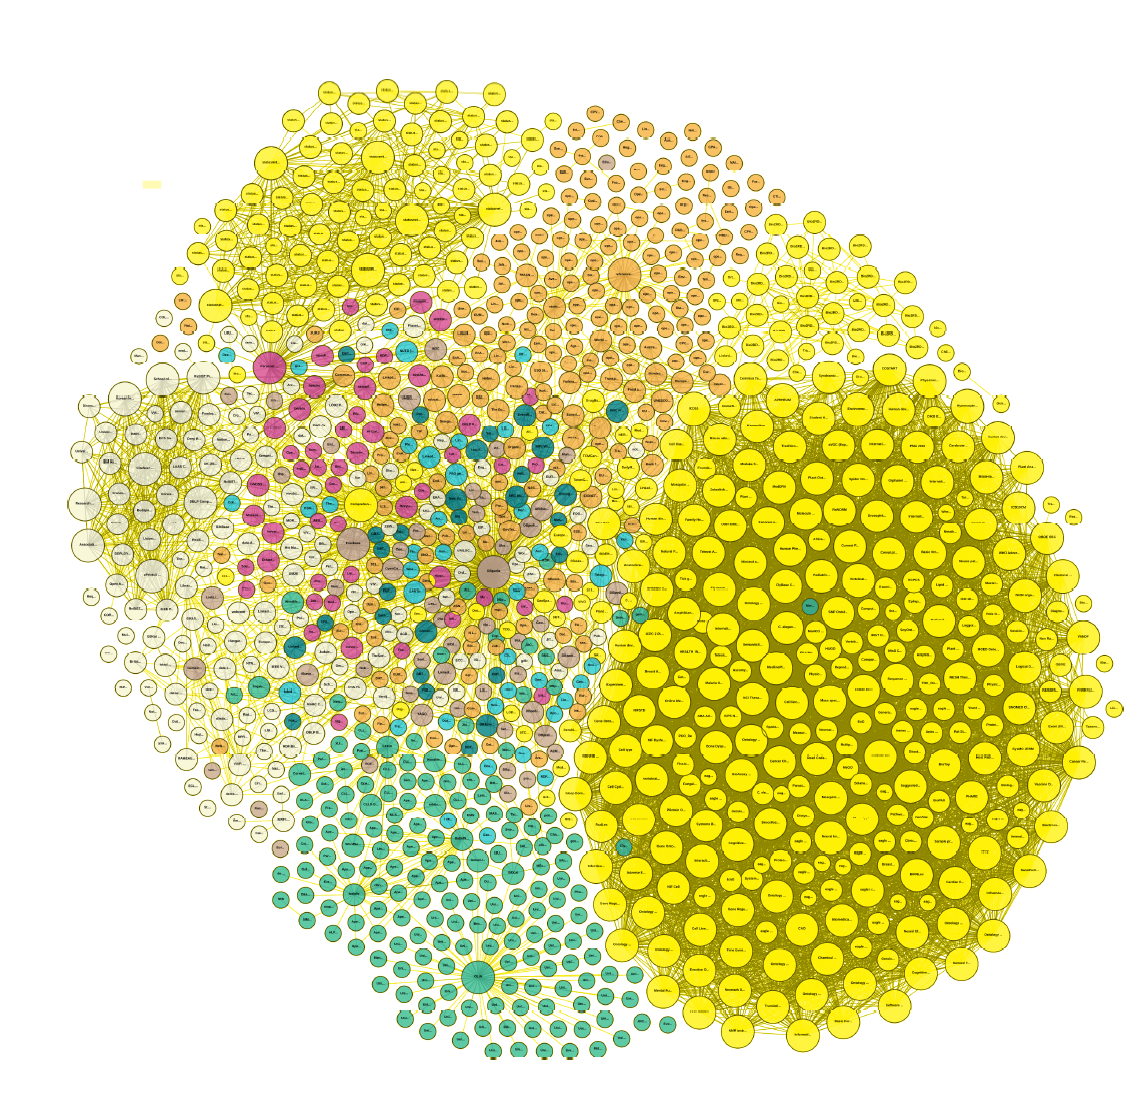
\includegraphics[width=1.55\textwidth]{images/chap02_LinkData.png}
		\end{minipage}
		\caption[Linked data diagram]{Linked data Diagram\cite{Hector}}
		
		
	\end{figure}
	
\end{center}
\subsection{RDF}
The Resource Description Framework (RDF) is a family
of W3C specifications. RDF is used to describe and model information. It describes as a subject that predicts an object is called a triple.
i) Subjects that RDF expressions describe them.
ii) predict is specific properties, attribute, or relation to describe a resource.
iii) The object is the name of property or value.
We can build a graph based on these three objects.

\subsection{SPARQL}
According to Wikipedia definition: It is a semantic query language for a dataset that makes us able to retrieve and modify data stored in RDF format.    

\subsection{Ontology Web Language }
Ontology Web Language is made to represent knowledge about things and the relations among them. OWL is a computational logic-based language, which means the language modeled in OWL can operate in a computer program like negation, intersection, and so on.

\section{Vocabularies}
\subsection{Vocabulary in Distributed Ledger}
To generate linked data, it requires to use a standard ontology or vocabulary to explain the blockchain concepts. Interfaces between distributed ledgers and the Semantic Web are still on an early stage. Some systems define such vocabulary such as FlexLedger, Ethan, BLONDiE\cite{Third}.\\

\textbf{\textit{FlexLedger}}: describes HTTP interfaces to blockchains, with a standard vocabulary and responses of these interfaces. FLexLedger is a protocol for decentralized ledger and graph data model which represents ledger creation, querying, and data model using JSON-LD. However, FlexLedger does not have explicit vocabulary about ontology nor having concrete ontology for itself. 
\\It is striking to say that the FlexLedger is not suitable to implement in some graph model like graph chain because in FlexLedger meta and the content data are stored together in the same graph whereas the GraphChain blocks’ content is stored outside the blockchain a separate graph \cite{Sopek}.\\

\textbf{\textit{EthOn}} is an OWl ontology that describes blockchain classes such as \textit{"blocks, accounts, message" ,"state"}and relations such \textit{"has parent block"}\cite{Rashid}. 
\begin{center}
	
	\begin{figure}[htb!]
		
		\begin{minipage}{0.50\linewidth}
			\centering
			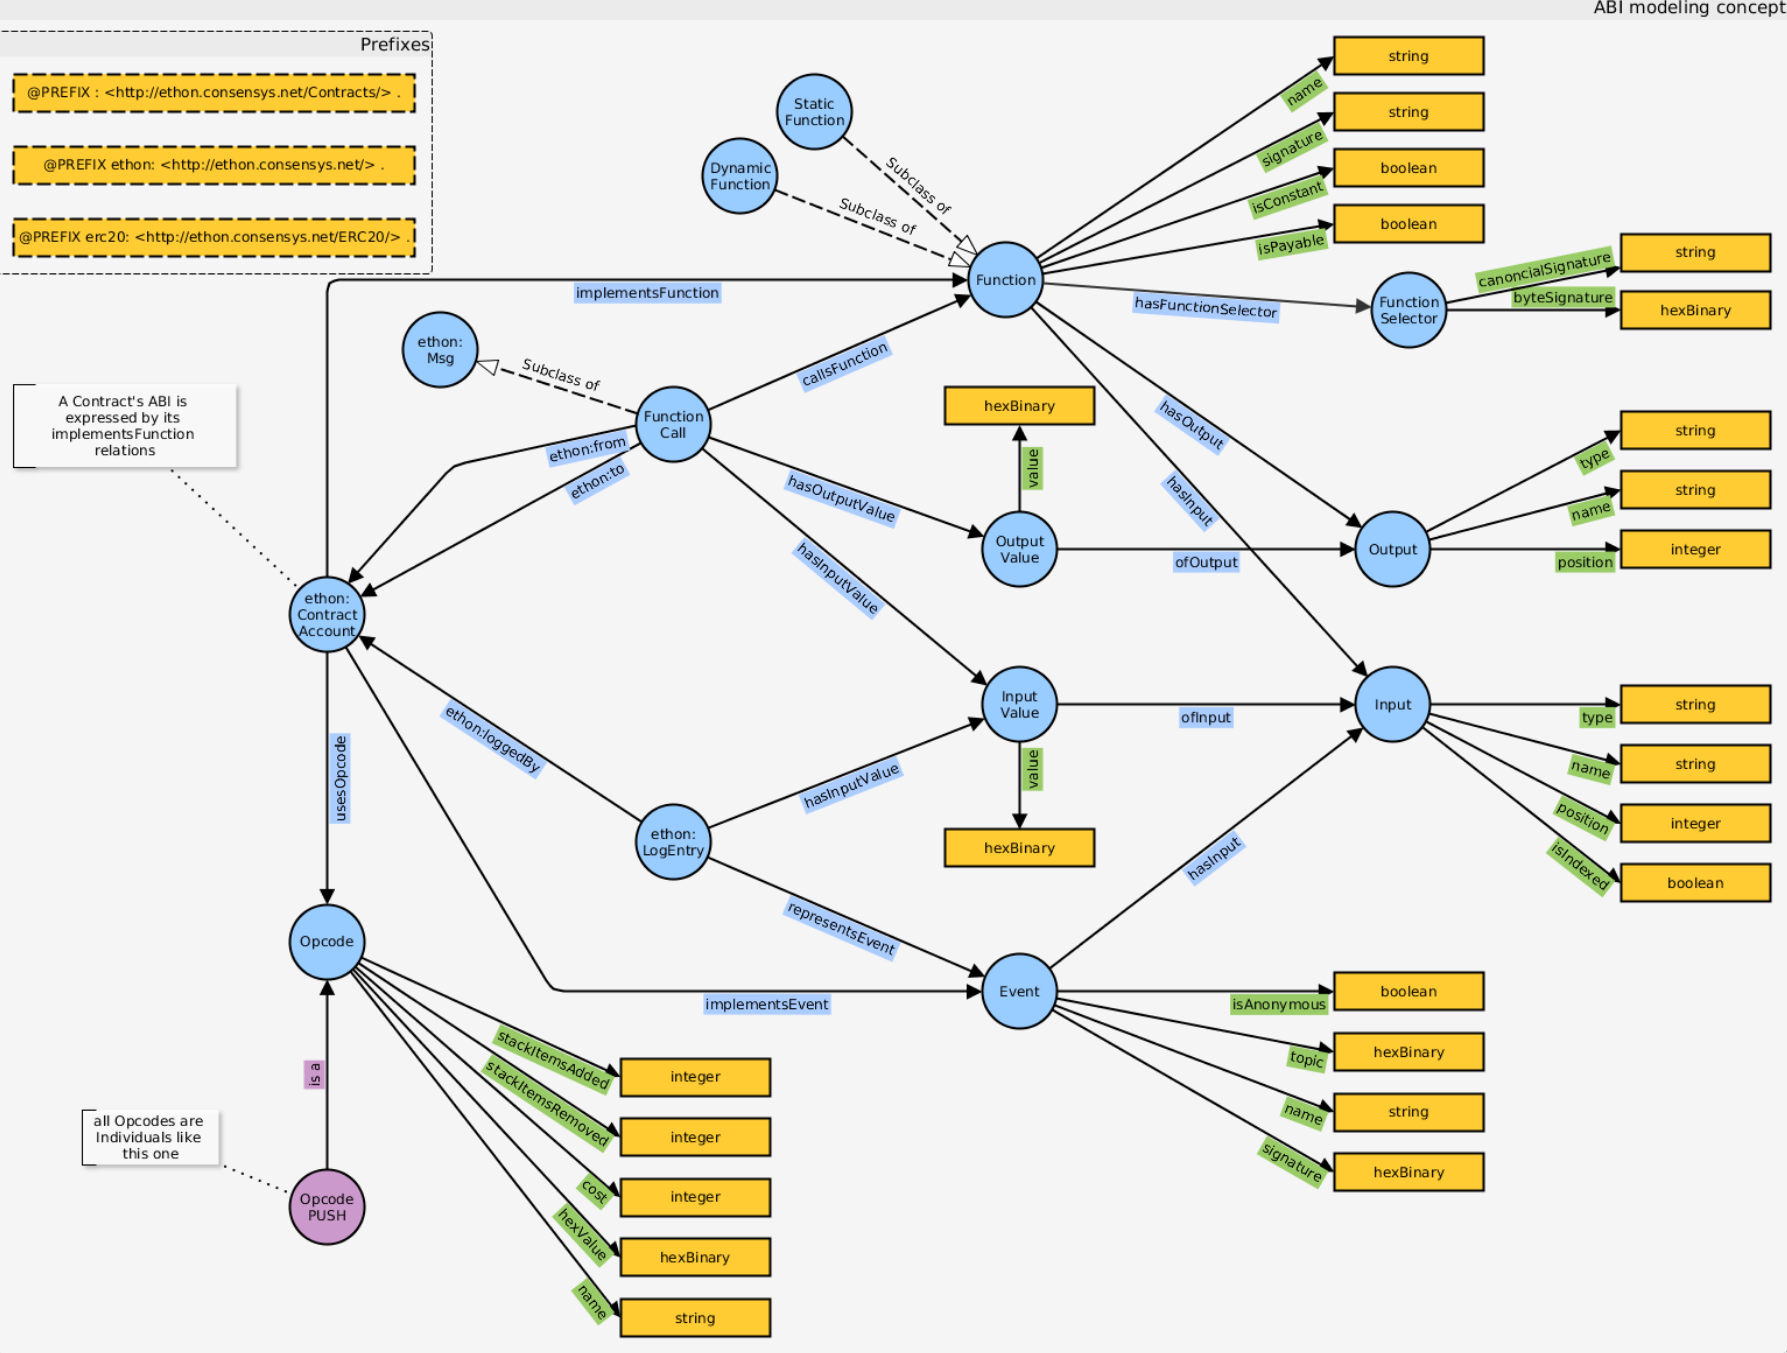
\includegraphics[width=1.80\textwidth]{images/chap2_EthOnContract.png}
		\end{minipage}
		\caption[EthOn classes]{EthOn Contract Model(blue arrow is object properties, green arrow is data properties, purple circle is instance and blue one is class)\cite{Rashid}}
		
	\end{figure}
	
	\begin{figure}[htb!]
		
		\begin{minipage}{0.55\linewidth}
			\centering
			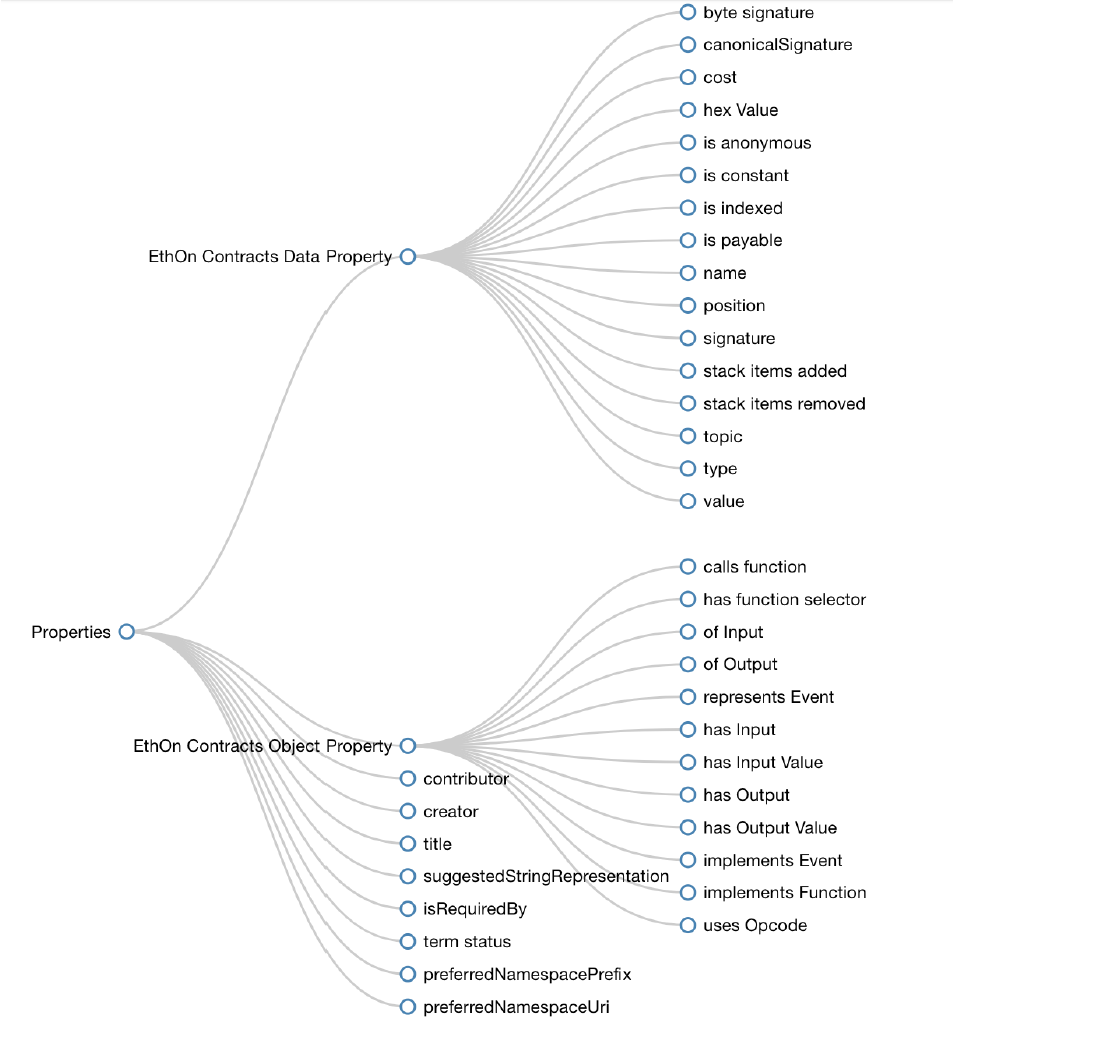
\includegraphics[width=1.65\textwidth]{images/chap02_EthOn_Properties.png}
		\end{minipage}
		\caption[EthOn Properties]{EthOn classes\cite{Rashid}}
		
		
	\end{figure}
	
\end{center}

\textbf{\textit{Blockchain Ontology with Dynamic Extensibility}}    
BLONDiE is another OWL ontology for describing the
Blockchain structure like EthOn. But, it is more generic then EthOn. For example, EthOn and BLONDiE both defined some terms such as 'account', 'block', 'transaction', and some attributes such as 'transaction payload' or 'miner address'. BLONDiE defines some other concept for different Blockchain such as 'BitcoinBlockHeader' and 'EthereumBlockHeader' as subclasses of 'BlockHeader'. At the moment, BLONDiE supports two cryptocurrencies like bitcoin and Ethereum where all links and relationships between objects and attributes represent in RDF(Resource Description Framework)\cite{Third}.
\begin{center}
	\begin{figure}[htb!]
		
		\begin{minipage}{0.55\linewidth}
			\centering
			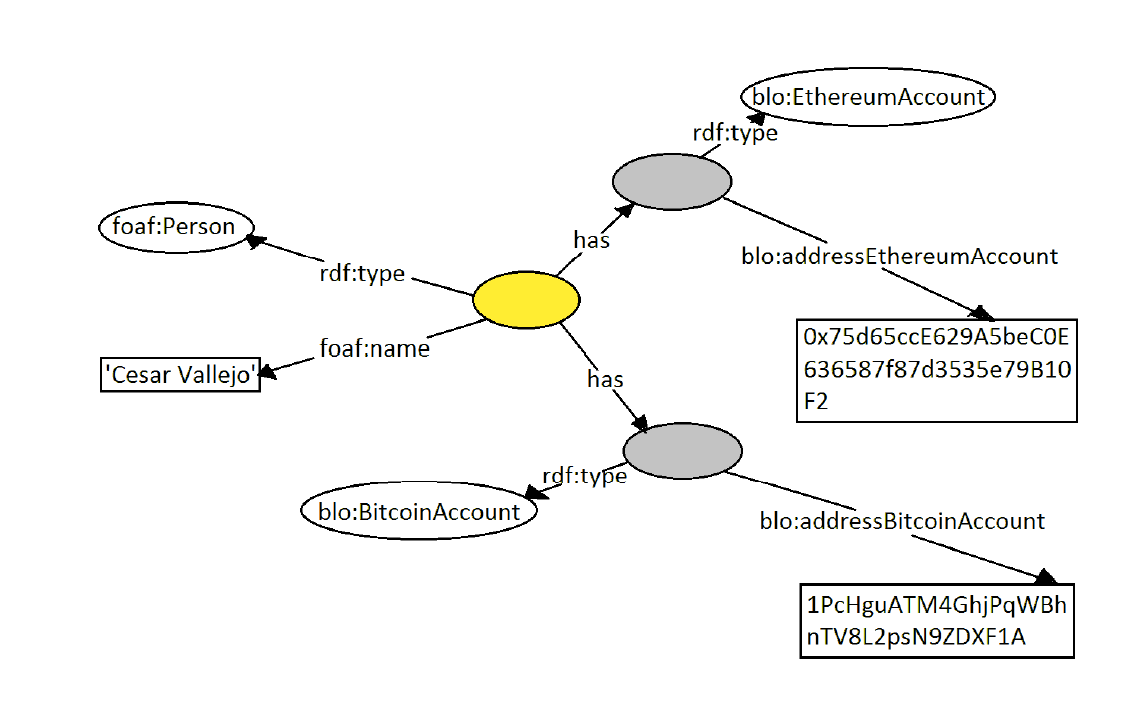
\includegraphics[width=1.75\textwidth]{images/chap02_BLONDiE.png}
		\end{minipage}
		\caption[BLONDiE]{BLONDiE usage example\cite{Hector}}
		
		
	\end{figure}
	
\end{center}
\subsection{Vocabulary in Smart Contracts}
As mentioned earlier, EthOn and BLONDiE are both similar concepts that can be used for smart contracts. As the smart contract is the executable software, so the semantic and vocabularies that are applicable for other software too.\\
There are many works on semantic annotation of the web and HTTP APIs which may enable us to annotate smart contracts as well. However, the contracts are not Web API and implementation may differ but the main concept does not differ. In other words, the vocabularies used to annotate web services, are used to annotate smart contracts too. It seems that the Combination of a distributed ledger with smart contract and web service due to profitability becomes common\cite{Third}.

\subsection{Ontology-based smart contract}
Kim and Laskowski\cite{Kim} propose ontology can help in the development of smart contract which can be executed on the blockchain. This approach can come up with proof of concept using Etheruem or other traceability ontology\cite{Hector}.

\subsection{Decentralized Storage and RDF}
The main goal of data over the web is to make a data machine-readable format on the web. It causes to interpret data in suitable formats to be useful in a way that is human readable too. \\
JSON-RPC is a remote procedure call protocol in JSON. This protocol allows sending data to the server without needing to the response. 
Ethereum blockchain which has properties such as pay fee with Gas. there are different ways of storing data in an RDF triple
The most wallet in Ethereum in JSON format that is easily convertible to RDF and front-end is made up of HTML  technology that we can use it to embed data on the website interface as Microdata, JSON-LD. The main focus of research is the storage of data on blockchain itself. There exist limitations of storage in Ethereum blockchain and fees. that's why it is suitable to use compact RDF serialization. There are some methods to store data on Ethereum blockchain that are summarized in the table below\cite{
	Hector}:\\

\begin{center}
	\begin{figure}[htb!]
		
		\begin{minipage}{0.55\linewidth}
			\centering
			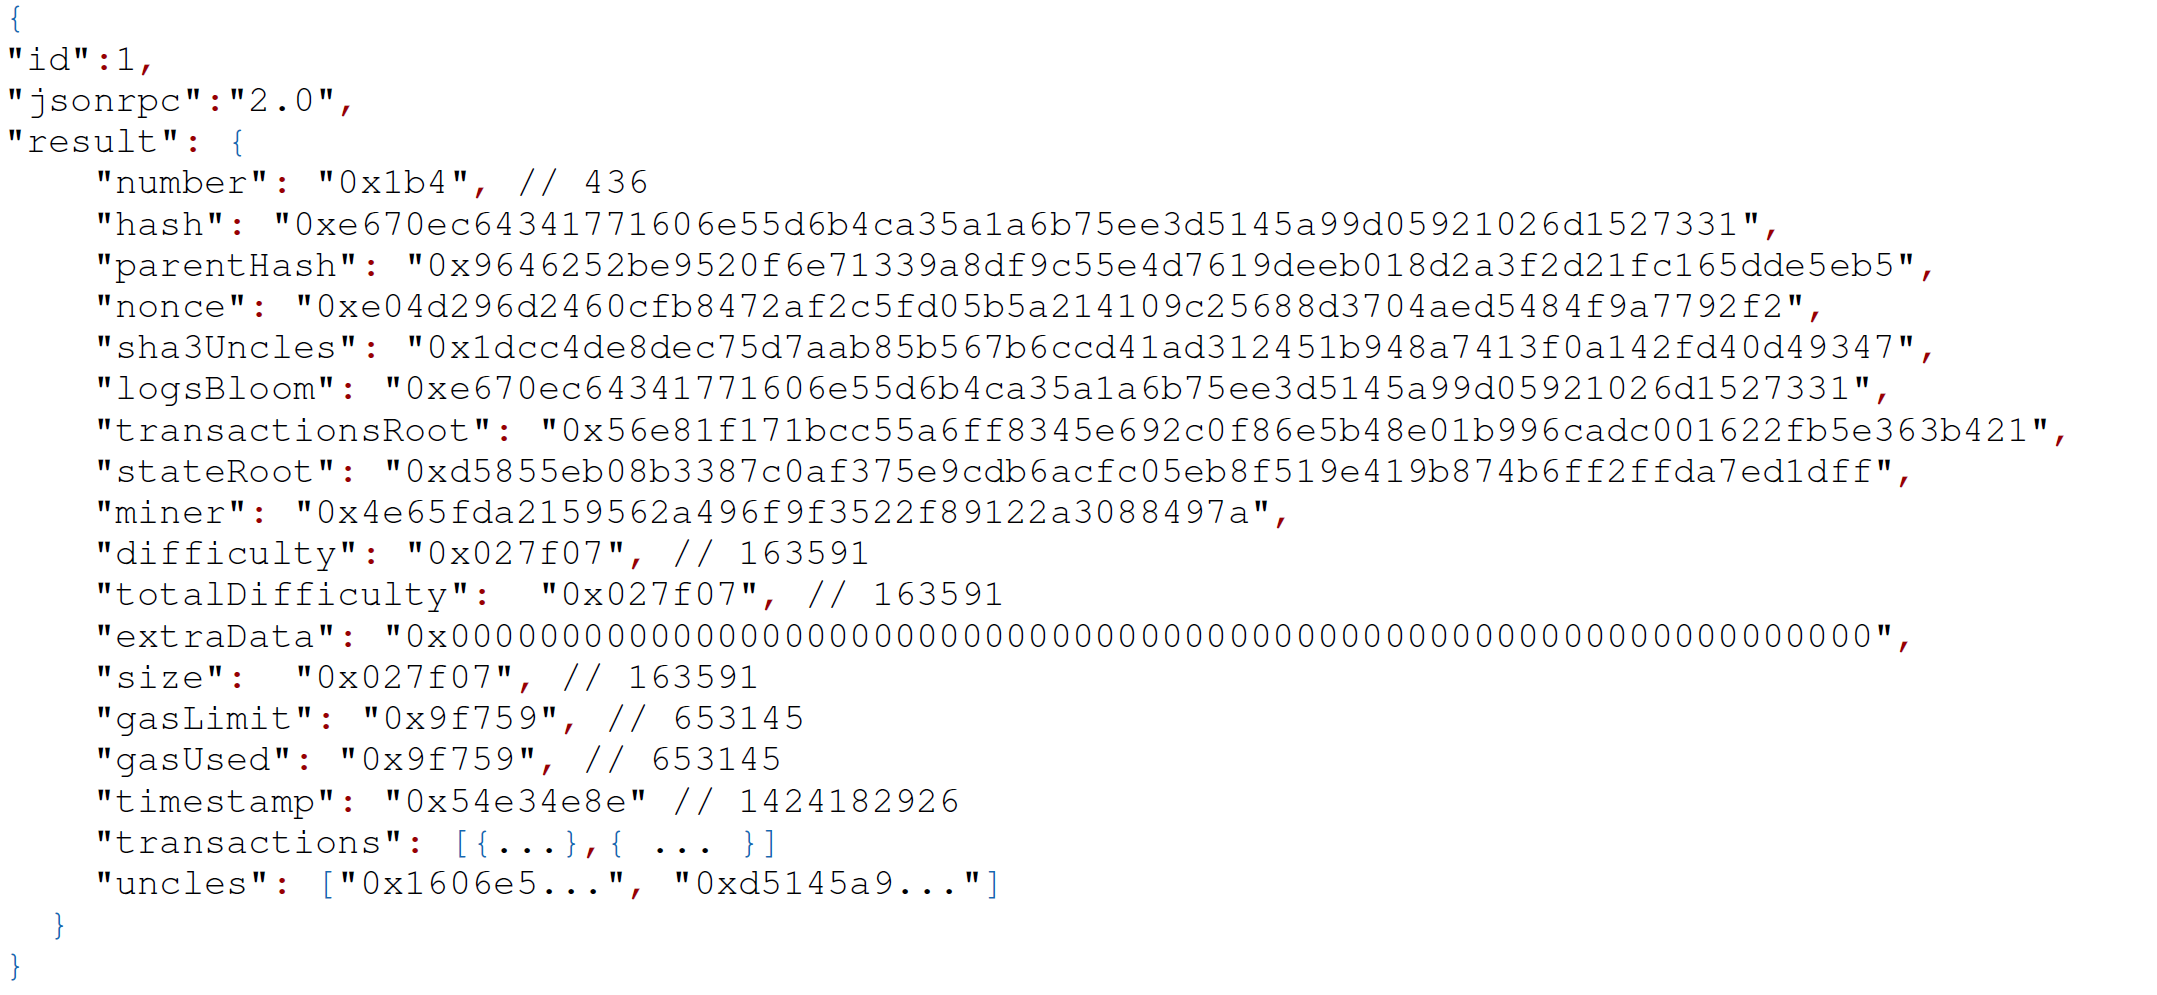
\includegraphics[width=1.95\textwidth]{images/chap02_Eth_str.png}
		\end{minipage}
		\caption[Ethreuem structure]{Ethereum structure}
		
	\end{figure}
	
\end{center}
\begin{center}
	\begin{figure}[htb!]
		
		\begin{minipage}{0.55\linewidth}
			\centering
			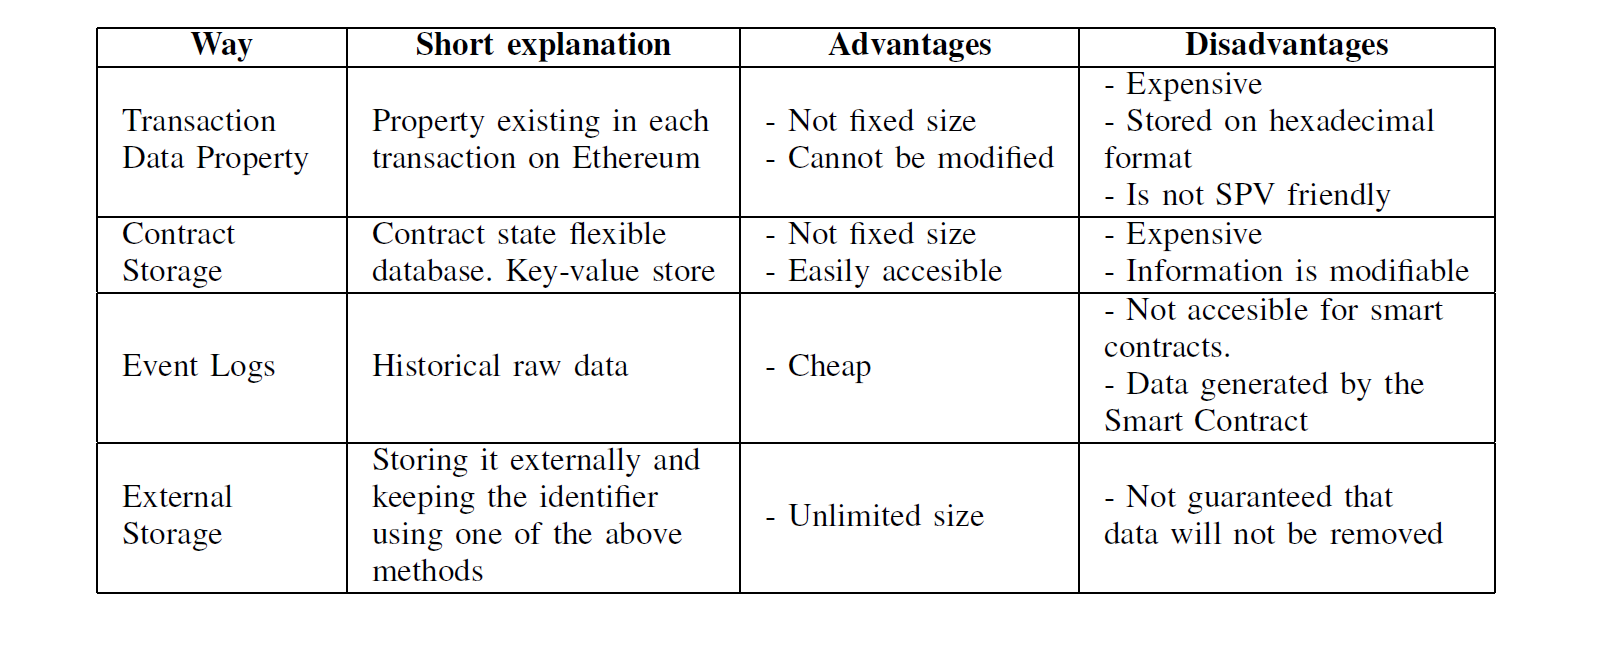
\includegraphics[width=1.95\textwidth]{images/chap02_Eth_Table.png}
		\end{minipage}
		\caption[Storage of RDF data on Ethreuem summery]{Storage of RDF data on Ethreuem summery\cite{Hector}}
		
	\end{figure}
	
\end{center}

\subsection{Semantic Blockchain}
By increasing the usage of blockchain technology recently, the need for semantic reasoning on the distributed ledger is on the crease as well. The blockchain is the best platform to utilize semantic web principles in this technology and add a new trusted property to a dataset. It makes a new dataset so trustworthy. 
Using semantic web technology on blockchain in a novel idea and the way of how to apply this technology in blockchain and smart contract is also an as controversial issue.\\
There are some \textbf{definition of semantic blockchain:}\\ 
\textit{Semantic blockchain is the representation of stored data on distributed ledger using linked data. }\\
\textit{Semtcic blockchain is the applying semantic web standard on the blockchain that these standards are based on RDF.}

\subsection{semantify Blockchain process}
Semantic blockchain or semantic distributed ledger affects the industrial world and subsequently, the result leads to start developing new application and framework to combine two worlds:
thee are some way to sanctify blockchain:
\textbf{-}Mapping the basic blockchain to RDF making usage of vocabulary, ontology, and so on.
\textbf{-} Storage of data in a blockchain is expensive, The only way is to store the hashing point to data set in blockchain and then share RDF on the blockchain.
\textbf{-} Create semantic blockchain that internal data exchange protocol is based on RDF\cite{Hector}.

\subsection{Semantic Ontology Mapping}
To generate RDF, it needs to map the basic blockchain entities to relevant semantic web terms, concepts, and ontology. To make the query more efficient, BLONDiE used some ways such as \\  
Firstly, records relating to block and transactions both, have been completed with an attribute for hashing to provide a direct mapping between contents of index and address of entities on the blockchain, Secondly, the transaction is strengthened with link some entities like blocks or smart contract and input to originating contract.\\
Blockchain stores just a binary form of each contract with metadata.   
it requires to have the relevant Application Binary Interface (ABI) specification in JSON form to interact with such a contract. This specification is created when the smart contract is compiled and stored in the blockchain and also smart contracts will index on the blockchain in binary form. To interact with contract Application Binary(ABI) Interface specification is needed. This specification is in the form of JSON and created when a smart contract is compiled and stored in the blockchain. The ABI determines all functions of contracts and descriptions about input, output parameter for each contract\cite{Third}.

\begin{center}
	\begin{figure}[htb!]
		
		\begin{minipage}{0.55\linewidth}
			\centering
			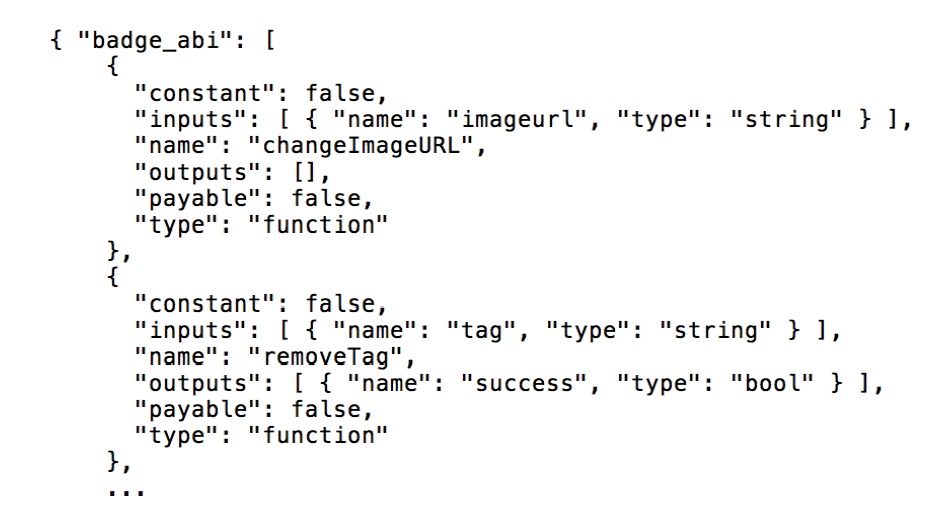
\includegraphics[width=1.95\textwidth]{images/chap02_SmartContract_ABI.png}
		\end{minipage}
		\caption[Smart contract of ABI]{Smart  contract of ABI}
		
	\end{figure}
	
\end{center}
By the presence of address and ABI, it is obvious to generate RDF to index smart contracts.
Allan Third at el.\cite{Third}model smart contract as follow:\\
- A contract as \textit{msm:Service}\\
- A function as \textit{msm:operation} with (\textit{msm:hasInput} or \textit{hasOutPut}) related to suitable \textit{msm:MessageContent}\\
- A msm:Service records contains the blockchain address as an attribute to keep the index into blockchain.

\subsection{Minimal Service Model}
The MSM defines a service that has Operations. Operations have input, output, and default MessageContent that may include mandatory or optional MessageParts. MessagePart provides support for finer-grained input/output discovery, as available in OWL-S and WSMO\cite{Rashid}.

\begin{center}
	\begin{figure}[htb!]
		
		\begin{minipage}{0.55\linewidth}
			\centering
			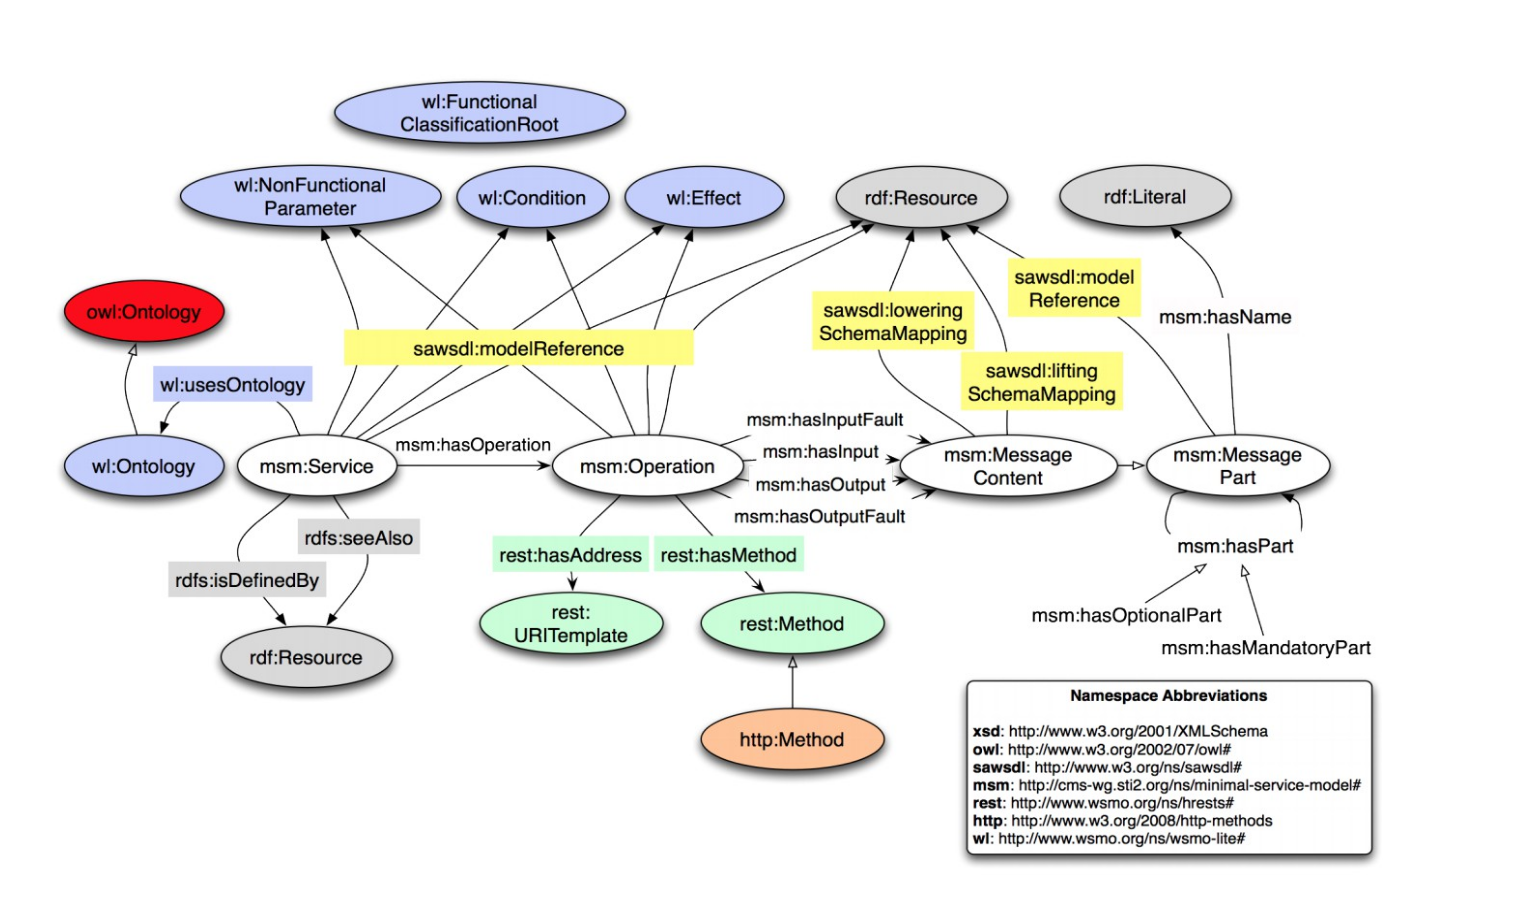
\includegraphics[width=1.95\textwidth]{images/chap02_MSM.png}
		\end{minipage}
		\caption[Illustration of Minimal Service ModelOntology]{Illustration of Minimal Service Model Ontology\cite{Rashid}}
		
	\end{figure}
	
\end{center}
We present one example that Rashid et al. used to clarify more the meaning of MSM in the blockchain: In this example, educational data is used to store in the blockchain using Ethereum \textit{web3} library.\\
it is considered that every block adds to blockchain and retrieve transaction within the block. If the transaction contains a smart contract. Then it retrieves the contract address using Ethereum API. Then, it saves the smart contract address, Application Binary Interface(ABI) as triple in RDF. ABI describes the name of smart contracts and way of calling them. Auther, then saved each method in ABI as an RDF triple based on MSM ontology as follow\cite{Rashid}:

\begin{center}
	
	\begin{tabular} { c | c }
		
		\textbf{Smart Contract Methods} & \textbf{MSM}\\
		\hline
		Smart Contract ABI & msm:service\\
		\hline
		Function   & msm:opreation\\
		\hline
		Input   & msm:messagecontent\\ 
		\hline
		Output   & msm:messagecontent\\ 
		\hline
		Gas   & msm:gas(from EthOn Contract DataProperty 'cost')
		
	\end{tabular}
	
\end{center}

\subsection{Web 3.0}\cite{Hector}
The evolution and interaction of people on the Internet
emerged on a classification of this revolutionary technology.
Early websites formed what is now known as Web 1.0 the
“web of documents”, documents serving as information portals
with basic ability to link websites. Later the Web 2.0 emerged
as the “web of people”, it introduced users to collaborate
with content creation and alteration. For the coming Web 3.0
there is a debate about what is the proper definition of its
characteristics. For some group, the Web 3.0 is powered by the
Semantic Web, where people can access to linked information
fast and easy. But now, with the emergence of a decentralized
web powered by Blockchain technology and since it enables
unmediated transactions, there is a new focus on the Web 3.0
based on the trustful nature of the blockchain. It is
the “read-write-own web”. Here, the user owns and participate
in owning the protocol. It is both peer to peer and machine
to machine. And it applies to people, companies, and
autonomous entities [14].
For instance, the term Web 3.0 is used by Ethereum in
a different context than the suggested by Berners-Lee. It is
proposed as the separation of content from the presentation
by removing the need to have servers at all [15]. Stephen
Tual, Ethereum’s CCO’s, defines that what makes Ethereum
different than Web 2.0 is that “there are no web-servers, and
therefore no middleman to take commissions, steal your data
or offer it to the NSA, and of course nothing to DDoS”.


\section{Retrieve Information form semantic blockchain}
Reasoning and knowledge representation in the semantic web is based on Description Logic(DL). Description logic has some elements such: classes and properties, the link between a different object, etc. Ontology is the study about the objects and relations between these objects or entities.
Each DL has a set of constructors to combine the concept and roles.
Concepts used in inclusion and definition axiom that model knowledge domain. These axioms called terminological box(TBox) concerning ontology individual axioms from Assertion Box (ABox). ABox and TBox create Knowledge Base(KB). \\
This study extends in the keeping with the retrieving the most relevant resources for a given query by the requester, where both query and resources are ontology-based and matched called semantic matchmaking. This process leads to two approach \textit{full match}, \textit{no match}. 
For request $R$ and resource check whether all features in request exist in $S$.
The classic inference service is capable of to Boolean match approach.
But, It is not enough because fully matched is rare. Non-standard inference determines the semantic ranking of resources concerning request and logic-based results.
If request and resource are not compatible:\\
-  contradiction concept which part $R$ is not compatible with $S$. Consider $G$ is the part that has conflict and $K$ as a part where $S$ and $R$ are compatible.\\
- Concept Abduction: $R$ and $S$ are compatible but $S$ not match fully with $R$.
consider $H$ as a Hypothesis that represents what is request in $R$ and not exist in $S$.
If $R$ and $S$ are not matched. Use contraction to represent $K$ part(compatible part) and $H$ hypothesis to suggest part to reach full match.\\
Moreover, we used the number of an element $G$ and $H$ in penalty function computation to define the semantic distance matrix.
This matrix can be used to rank resources concerning request\cite{Ruta}. 

\subsection{Semantic Blockchain Architecture} 
This method purposed a framework based on the semantic discovery layer built upon basic blockchain. It is striking to see the main features of such a blockchain as follow:

\begin{center}
	\begin{figure}[htb!]
		
		\begin{minipage}{0.55\linewidth}
			\centering
			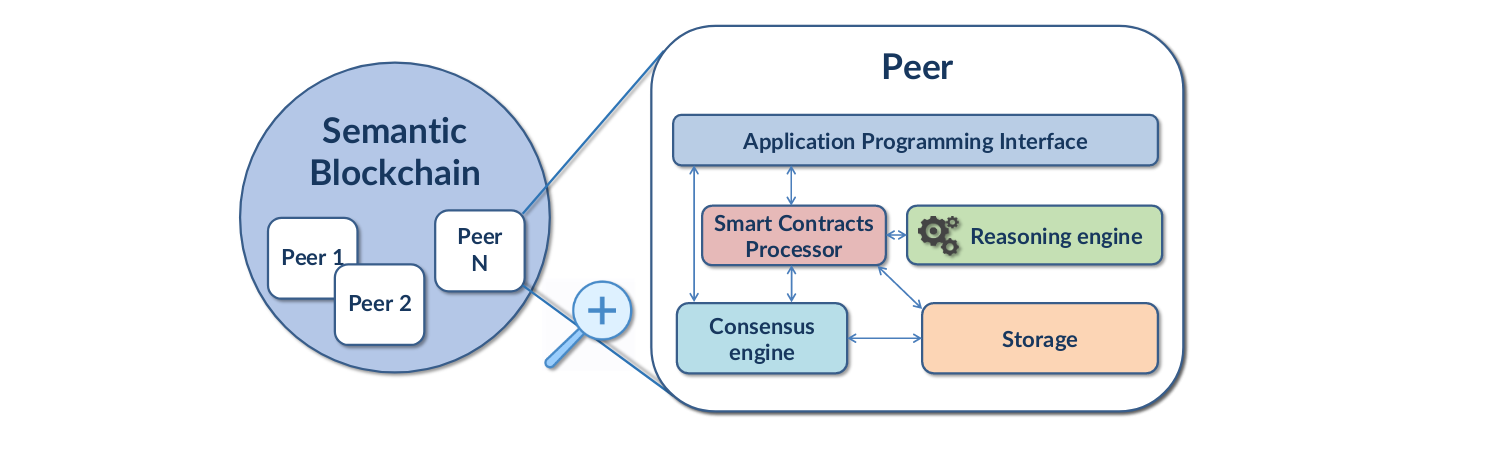
\includegraphics[width=1.95\textwidth]{images/chap02_PeerBlockchain.png}
		\end{minipage}
		\caption[Framework Arciteture]{Framework Architecture \cite{Ruta}}
		
	\end{figure}
	
\end{center}


\textbf{Peer} agent is identified as by public key and its accounts. Each agent can enforce semantic discovery to transfer assets between annotations that are stored in the blockchain. And each peer is integrated of matchmaking and reasoning engine for semantic discovery.

\textbf{Asset} represents the resources and service instances based on domain ontology.\\
\textbf{Smart Contracts} are the integration of matchmaking and reasoning engine.\\
\textbf{Consensus Engine} allows to validate transaction in blockchain.\\
\textbf{Storage} built up  \textit{markle tree} out of transactions including semantic ones to efficient detection of erroneous change in transaction\cite{Ruta}.

\subsection{Making smarter Contract: Putting Semantic in Consensus Protocol}

In the semantic blockchain, EthOn or BLONDiE concepts and vocabulary to facilitate integrity and develop resource discovery. EthOn concept used W3CRDF schema and web ontology language to describe blockchain contract concepts. By the use of these concepts, it is possible to compare requests with different recourse concerning semantic annotation of shared domain ontology. \\
Smart contract semantic is represented by a service layer that gives a correct description of discovery outcome. Thus, it raises the trust of the discovery process for users. In the semantic blockchain, Baqa et al.\cite{Baqa} used domain ontology to maps to EthOn contract. These concepts used for OWL-S ontology, indexing, and invoking smart contracts on Blockchain via URIs\cite{Baqa}. 
Semantic blockchain also performs operations such as registration, discovery, selection, and execution that are implemented as a smart contract. \\
Ruta at el.\cite{Ruta} focused on semantic mismatching as a significant feature of semantic blockchain concerning basic blockchain. This allows computing the semantic distance between resources and queries with the same ontology.
The logic-base matrix enforces the semantic ranking of the element of the query\cite{Ruta}. \\ 
\textbf{A: Resource Registration:}
As already mentioned, a Smart contract designed using OWL specification. It used concepts and entities defined as a class in OWl language and relationship between entities defined as object properties concerning ontology. To construct smart contract semantic requires a framework to design such contracts.\\
Multiple resources stored on the blockchain and Each domain is related to a different ontology that provides vocabularies for annotating resources. Resources also are categorized by attributes such as URI of reference ontology to retrieve the resource, semantic annotation in OWL that describes resources, resource price.\\
To register resources on the blockchain, 
a user is required to register an account with public address and related private key to call the smart contract as a parameter. 
In ontology, a user describes as class corresponding to an account along with other attributes such as an address, private key, and other details. \\
To achieve this, A new ontology called \textit{EthereumContractConcepts} is implemented containing \textit{EthereumContract} data property. A \textit{ContratcAccount}
consist of license number, date, smart contract owner and state.
After all, a smart contract is developed with vocabulary as domain-based-ontology\cite{Baqa}.  


\begin{center}
	\begin{figure}[htb!]
		
		\begin{minipage}{0.55\linewidth}
			\centering
			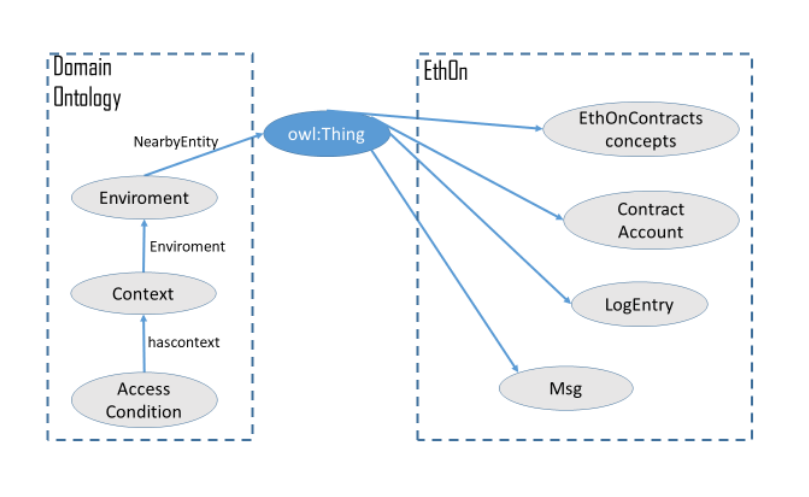
\includegraphics[width=1.95\textwidth]{images/chap02_Domain_EthOn.png}
		\end{minipage}
		\caption[Domain ONtology]{Domain ontology \cite{Baqa}}
		
	\end{figure}
	
\end{center} 

\textbf{B: Smart Contract}
EthOn and OWl concepts used to build semantic web service for smart contracts. OWL-S ontology is used that makes functionalities such discover, invoke, and monitor by providing some additional vocabulary along with smart contract concepts to facilitate query to finding a smart contract. The OWL-S ontology provides three types of description about service as follow: \\


\begin{center}
	\begin{figure}[htb!]
		
		\begin{minipage}{0.55\linewidth}
			\centering
			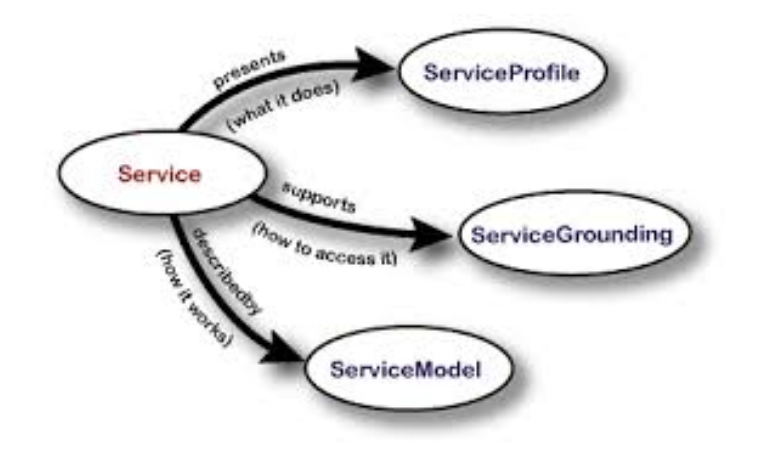
\includegraphics[width=1.55\textwidth]{images/chap02_SmartContract.png}
		\end{minipage}
		\caption[Service-based smart contract]{Service-based smart contract}
		
	\end{figure}
	
\end{center}
By the use of EthOn concepts, we can monitor added block to the blockchain. When a transaction has a smart contract, it is retrieved from the store contract address via API, then the address of smart contract and Application Binary Interface(ABI) as a triple in the RDF store. ABI consist of the smart contract method and way of calling it. Methods are stored in ABI as an RDF triple concerning OWL-S ontology. The table below shows the OWL-S vocabulary to describe smart contract\cite{Baqa}.
\begin{center}
	\begin{figure}[htb!]
		
		\begin{minipage}{0.55\linewidth}
			\centering
			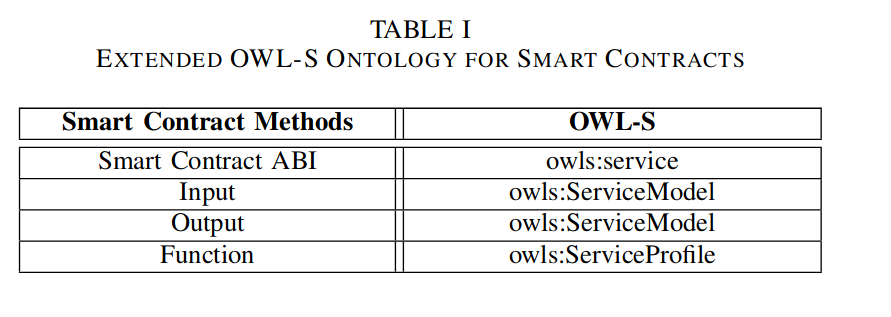
\includegraphics[width=1.95\textwidth]{images/chap02_OWL.png}
		\end{minipage}
		\caption[OWLS ]{OWLS ontology for smart contract} 
		
	\end{figure}
	
\end{center}
\textbf{B:Semantic Discovery }
To search for a smart contract or an item, The requester sends the request to $n$ nodes randomly specifying:\\
- URI of domain ontology to determine resource and vocabulary of both resource and request which to be retrieved.\\
- Semantic annotation of smart contracts in OWL language. \\
- Maximum Price $p_max$ that requester pays.\\
- Minimum semantic $s_min$ threshold in $[0,1]$ interval, 1 is related to full match and 0 is the mismatch. 
- maximum result $r_max$ is to be returned.
- Address of requester. \\ 
Baqa et al. here used the $gossip$ approach to propagate the request. The nodes which received the request perform 2 operations at the same time: First, preform semantic matchmaking of own resource with the request and provides a list of max result $r_max$ satisfying both semantic relevance score $s_min$ and cost $p_i <= p_{max}$, is returned.\\
Second, send the request to other $n$ nodes randomly, the other nodes perform in the same way until reach the $m$ thresholds. the request continue until reach the $\sum_{i=1}^{m} n^i$ with $n$ and $n$ parameters. Then do not forward the request and perform matchmaking locally.\\
Afterward, the nods send back the result to the main requester at the specified address\cite{Baqa}.\\

\textbf{C: Explanation} In this process, the requester sends the request containing: Semantic is the annotation of request and URI od related resource. The receiver node response matchmaking result that encompasses the semantic dependency score in [0,1]interval and the concept expression of G (conflicting part between R and S), K(the compatible part between R and S), and H(the hypothesis concept to reach the matchmaking). This process is optional and needed when the requester needs the explanation of matchmaking results.

\textbf{C: Resource Selection:} After receiving all results, the requester selects the best resource and smart contract, sending a message to the resource owner and contextually payment. the receiver responses with the proper resource representation relied on the meaning of uri[4].
The resource discovery and retrieval interaction are shown bellow and Each associated transaction is recorded on the blockchain\cite{Ruta}.


\begin{center}
	\begin{figure}[htb!]
		
		\begin{minipage}{0.55\linewidth}
			\centering
			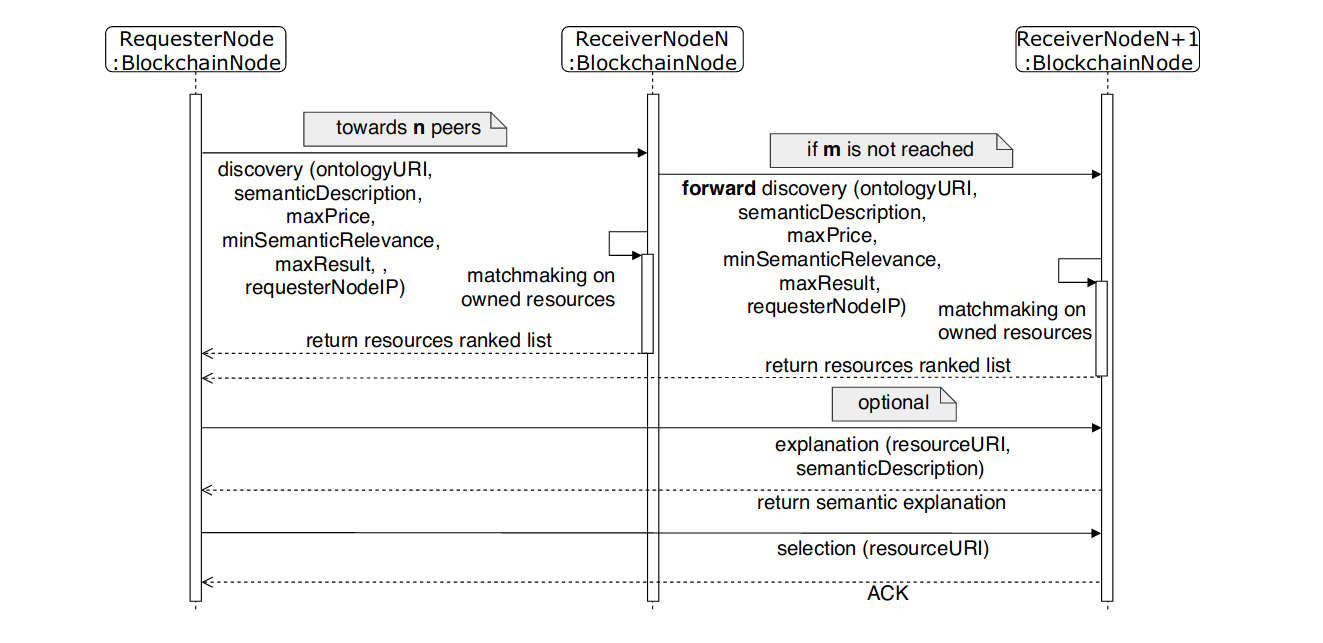
\includegraphics[width=1.95\textwidth]{images/chap01_SemanticBlockChain.png}
		\end{minipage}
		\caption[Resourse Discovery]{Resource Discovery\cite{Ruta}}
		
	\end{figure}
	
\end{center}

\subsection{Indexng of Smart Contract}
As already mentioned, the distributed ledger does not have a central registry due to its structure. The contract in this distributed ledger is not directly queried.
and blockchain is the time-ordered structure where data exist on multiple blocks.
In such a distributed structure, developing the indexing process for the smart contract is necessary. The indexing system provides the ability to analyze and search service on blockchain and displays the outside.
There is a different level of indexing such as low level to index basic entities such as account, transaction, block and the top level for more functional operations is indexed.

\subsection{EthOn}
Is an ontology that describes blockchain concepts such as transaction, account, block using w3RDF
schema and ontology web language OWL to describe the relation of these objects on the blockchain.
To model data and be understandable for resource, EthOn and some semantic such as "hasParentBlock".
EthOn in at infancy and should develop more to have smart contract concepts, functions, events, input, and output, etc.
EthOn accepts consider just some relation between smart contract and Ethereum framework. Some multiple tools and languages can annotate a smart contract. In this study, It is focused on OWL-S ontology due to some significant features such as flexibility, wide description of service, and no- restriction... 
The main goal is to develop to support the smart contract too for semantic web service context.
For reaching this aim, the web graph chain is PI and a smart contract can be represented as an executable function in a distributed environment. The semantic web describes message, service, and entities in a machine-readable format that can support logical reasoning based on semantic web service description. It helps to map between different ontologies that facilitate the transformation of the concepts among ontologies\cite{Baqa}. 

\begin{center}
	\begin{figure}[htb!]
		
		\begin{minipage}{0.55\linewidth}
			\centering
			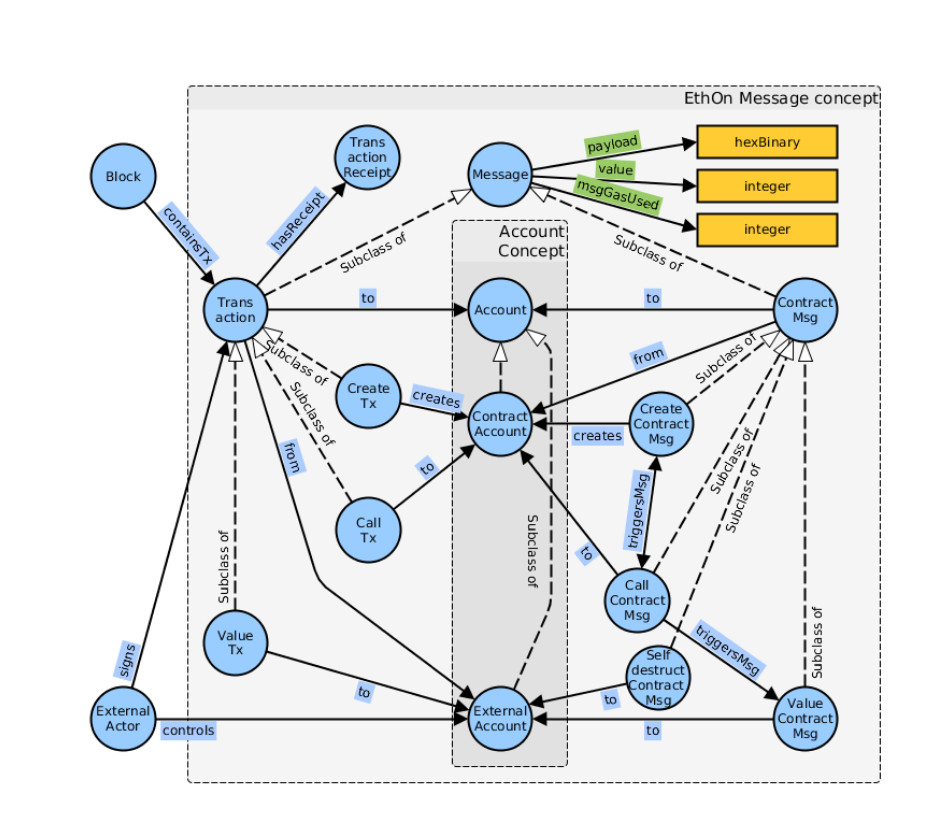
\includegraphics[width=1.65\textwidth]{images/chap02_EthOn.jpg}
		\end{minipage}
		\caption[EthOn message concept]{EthOn message concept\cite{Baqa}}
		
	\end{figure}
	
\end{center}



